\documentclass[11pt, a4paper]{report}

% Packages
\usepackage[utf8]{inputenc}
\usepackage[T1]{fontenc}
\usepackage{amsmath}
\usepackage{graphicx}
\usepackage[colorlinks=true, linkcolor=black, urlcolor=blue, citecolor=blue]{hyperref}
\usepackage{fancyhdr} 
\usepackage{titlesec}
\usepackage{xcolor}
\usepackage{enumitem}
\usepackage{wrapfig}
\usepackage{booktabs}
\usepackage{float}
\usepackage{comment}
\usepackage{subcaption}
\usepackage{xurl}

% Formatting
\usepackage[
a4paper,
top=2cm, 
bottom=2cm,
inner=2cm,
outer=2cm,
marginparsep=0.5cm,
showframe=false
]{geometry}

\setcounter{tocdepth}{1}

\usepackage{setspace}
\onehalfspacing

\usepackage{times} % Times-like serif font
\usepackage{mathptmx} % Match math to Times

% Chapter titles format
\titleformat{\chapter}[hang] % Use 'hang' format, which prints title on one line
{\normalfont\bfseries\Huge} % Font style (Bold, Huge size)
{\thechapter} %{\chaptertitlename\ \thechapter:} = "Chapter 1:"
{1em} % Horizontal space between label and title
{}
\titlespacing*{\chapter}
{0pt}{3.5ex}{2.3ex} % {left}{before skip}{after skip}

\begin{document}
	\begin{titlepage}
		\centering
		{\Huge \textbf{Semester project on signals in robot systems} \par} % Title of the report
		\vspace{1.5cm}
		
		{\LARGE BEng in Robot Systems \par} % Education
		\vspace{0cm}
		
		{\Large 3. Semester \par} % Semester
		\vspace{1.5cm}
		
		{\Large \textbf{Authors (Group 3)} \par} % Authors section
		\vspace{0.5cm}
		
		\begin{tabular}{l l l}
			Name & Username & Date of birth \\ 
			\hline
			Noah V. Vryens & novry24 & 01/04/2002 \\
			Rasmus K. Nielsen & rasni19 & 25/12/1997 \\
			Emma B. Rasmussen & erasm24 & 15/05/2001 \\
			Jannick H. Irvold & jairv24 & 23/10/2002 \\
			Eymundur Ó. Pálsson & eypal24 & 31/08/2002 \\
		\end{tabular}
		\vspace{2cm}
		
		{\Large \textbf{Supervisor} \par}
		\vspace{0.5cm}
		
		Cheng Fang \par
		chfa@mmmi.sdu.dk \par
		\vspace{10cm}
		
		Characters: 47.689
		
		\vfill
		
		{\large \today} % Date
	\end{titlepage}
	
	\pagenumbering{gobble}
	
	In this project, the goal was to balance an inverted pendulum attached to a cart, driven by a belt. To achieve stable balancing of the pendulum, mathematical models of the system were developed using both the Newton-Euler and Euler-Lagrange methods. The resulting dynamic models were linearized around the upright equilibrium position and used for simulation and controller development in MATLAB/Python. 

In addition to simulation, the project also focuses on implementation aspects related to real automation systems. This includes communication between software and hardware, PLC-based control implementation, and validation of the simulated models using the physical setup and tests. The project therefore demonstrates both the theoretical and practical challenges associated with modelling and controlling unstable dynamic systems in modern automation engineering. 

The modeling, controller design and implemented resulted in three controllers using different strategies, which all managed to stabilize the inverted pendulum. Though the controllers were stable, the physical performance did not fully match simulated results, likely due to unmodelled physical effects such as static friction, backlash, sensor noise, filtering delays actuator saturation and small mechanical imperfections in the setup.
	
	\tableofcontents
	
	\clearpage
	\pagenumbering{arabic}
	
	% Main Body (Chapters)
	\clearpage
\chapter{Introduction}
\label{chap:introduction}

In life and industri that are alot of machinery that need regualted and precice controll, which i why a controller is made to achive each goal as needed. In robotics controllers can be expicaly usefull when trying to complete difficult taskes with multipul moveing parts. Where balance is one of main hindrences, when trying to design such a system. This projeckt will focus trying to solve a balance isuee of an inverted pendulem. 

\section{Project Goals}

With a PLC, motor, conveyor track, inverted pendulem on a cart and a two diffrencet controller. it is attempted to make the inverted pendulem balance rightsideup using a controller to controll the force of the motor. success is mesurd by how well the controller balences the pendulem compared to a simulation of the controller, and the best controller is the one whose closest to the simulation of said controller.

   
\section{Problem Definition}



\section{Constraints \& Limitations}
The limitations for this projeckt come from the physical setup, and the PLC. The cart is limited to move within two sensors on the conveyor track, and the maximum force for the moter is X. For the PLC it cant run faster than 1000Hz, and sampling via OPCUA is limited to 100Hz



\section{System OverView}

	\chapter{System modeling}
\label{chap:system modeling}
\section{Modelling of the Inverted Pendulum System}

\subsection{System description}

The purpose of the modelling process is to obtain a mathematical representation of the inverted pendulum system, which can later be used for simulation and controller design. A mathematical model makes it possible to analyze the dynamic behavior of the system and evaluate different control strategies before implementation on the physical setup.

In this project, two classical modelling approaches were used: the Newton-Euler method and the Euler-Lagrange method. Both methods describe the dynamics of the system, but from different physical perspectives. The Newton-Euler method is based on force and moment balances, while the Euler-Lagrange method is based on the kinetic and potential energy of the system. The resulting nonlinear equations were linearized around the upright equilibrium position to simplify the controller design and implementation in MATLAB/Python.

The physical system consists of a cart with an attached inverted pendulum with an additional weight mounted on top of it. The cart is constrained to move horizontally along a conveyor-driven rail, while the pendulum is free to rotate around its pivot point. The system is actuated by an external force $F$, which controls the horizontal movement of the cart. The goal of the system is to keep the pendulum balanced in its upright position while controlling the motion of the cart.

The generalized coordinates used to describe the system are:

\begin{itemize}
	\item $x$: horizontal cart position
	\item $\theta$: pendulum angle relative to the vertical axis
\end{itemize}

The following assumptions were made during the modelling process:

\begin{itemize}
	\item The pendulum rod is considered rigid
	\item Friction is assumed to be small and primarily represented by damping coefficients
	\item The pendulum motion is constrained to a two-dimensional plane
	\item The system is linearized around the upright equilibrium position
\end{itemize}

\begin{figure}[H]
	\centering
	\includegraphics[width=0.4\textwidth]{Figures/system_model.png}
	\caption{Simplified model of the inverted pendulum system showing the generalized coordinates, pendulum angle, and input force.}
	\label{fig:system_model}
\end{figure}

\begin{table}[H]
	\centering
	\caption{System parameters}
	\begin{tabular}{|l|c|}
		\hline
		Parameter & Value \\ \hline
		Mass of cart & 0.5 [kg] \\ \hline
		Mass of rod & 0.082 [kg] \\ \hline
		Mass of attached weight & 0.002 [kg] \\ \hline
		Mass of pendulum & 0.084 [kg] \\ \hline
		Length of rod & 0.35 [m] \\ \hline
		Length of conveyor belt & 1.72 [m] \\ \hline
		Radius of belt rollers & 0.05 [m] \\ \hline
		Gravitational acceleration & 9.82 [m/s$^2$] \\ \hline
		Linear damping coefficient & 5 [N/(m/s)] \\ \hline
		Rotational damping coefficient & 0.0012 [Nm/(rad/s)] \\ \hline
	\end{tabular}
	\label{tab:parameters}
\end{table}

\subsection{Newton-Euler Modelling}

The Newton-Euler method is based on applying Newton’s second law and rotational moment equations to the system. Free body diagrams were constructed for both the cart and the pendulum to identify the forces and moments acting on the system.

\begin{figure}[H]
	\centering
	\includegraphics[width=0.4\textwidth]{Figures/free_body.png}
	\caption{Free body diagram of the inverted pendulum system showing the applied force, gravitational forces, damping effects, and normal force acting on the system.}
	\label{fig:fbd}
\end{figure}

For the cart, the sum of forces in the horizontal direction was established using Newton’s second law:

\begin{equation}
	\sum F_x = M\ddot{x}
\end{equation}

The obtained equations contain nonlinear trigonometric terms originating from the pendulum rotation. To simplify the controller design, the equations were linearized around the upright equilibrium position using the small-angle approximations:

\begin{equation}
	\sin(\theta) \approx \theta
\end{equation}

\begin{equation}
	\cos(\theta) \approx 1
\end{equation}

\subsubsection{Final Linearized Model}

\begin{equation}
	(I + ml^2)\ddot{\theta} - mgl\theta = ml\ddot{x}
\end{equation}

\begin{equation}
	(M+m)\ddot{x} + b\dot{x} - ml\ddot{\theta} = u
\end{equation}

\subsubsection{State-Space Representation}

\begin{equation}
	\dot{x} = Ax + Bu
\end{equation}

\begin{equation}
	y = Cx + Du
\end{equation}

% INSERT FULL MATRICES HERE

\subsection{Euler-Lagrange Modelling}

The Euler-Lagrange method describes the system dynamics using energy relationships instead of direct force balances.

The kinetic energy of the cart is given by:

\begin{equation}
	T_{cart} = \frac{1}{2}M\dot{x}^2
\end{equation}

Using the derived expressions for kinetic and potential energy, the Lagrangian was formulated as:

\begin{equation}
	L = T - V
\end{equation}

The equations of motion were then derived using the Euler-Lagrange equation:

\begin{equation}
	\frac{d}{dt}
	\left(
	\frac{\partial L}{\partial \dot{q}_i}
	\right)
	-
	\frac{\partial L}{\partial q_i}
	=
	Q_i
\end{equation}

\subsection{Comparison of the Methods}

Both modelling approaches resulted in equivalent dynamic models after linearization, verifying the correctness of the derivations.

The Newton-Euler method provided a more intuitive understanding of the physical forces and moments acting on the system, since it directly uses force and torque balances. However, the method becomes increasingly complex for systems with multiple interconnected bodies.

The Euler-Lagrange method provided a more systematic and compact mathematical formulation by describing the system through energy relationships.

The final linearized model was implemented in MATLAB/Python and used for simulation and controller development. The derived model forms the basis for the PID controllers, pole-placement controller, and the discrete implementation used later in the project.
	\chapter{Control theroy}
\label{chap:control theroy}

\section{LQR controller}
One way to stabilize the inverted pendulum in its upward position, is a Linear Quadratic Regulator (LQR). LQR is an "optimal" multivariable controller that determines the best possible feedback gains by balancing the trade off between keeping the system states close to zero and minimizing the control effort used to do so.

\subsection{Discretization for PLC}
Because the controller will be running on a B\&R Programmable Logic Controller (PLC) running at a fixed cycle time of $T_s = 0.001$ seconds, the continuous time statespace model cannot be used directly.\newline
The system matrices are first discretized using a Zero-Order Hold (ZOH) method. This converts the physical model into a discrete-time representation that aligns with the digital sampling of the PLC.

\subsection{The Cost Function and Weighting Matrices}
The discrete LQR algorithm computes an optimal gain matrix $K$ by minimizing the discrete quadratic cost function:

\begin{equation}
	J = \sum_{k=0}^{\infty} \left( x_k^T Q x_k + u_k^T R u_k \right)
\end{equation}

Where:
\begin{itemize}
	\item $x_k$ is the state vector at time step $k$, defined as $x = [x_c, \dot{x}_c, \theta, \dot{\theta}]^T$.
	\item $u_k$ is the control input (motor force).
	\item $Q$ is a matrix that penalizes deviations in the system states (position and velocity errors).
	\item $R$ is a matrix that penalizes the use of the actuator (control effort).
\end{itemize}

\subsection{Tuning with Bryson's Rule}
Deciding what to put in the $Q$ and $R$ matrices in an intuitive way, Bryson's Rule is applied. This method scales each parameter based on its maximum acceptable physical limit, ensuring every variable contributes evenly to the cost function.\newline

The maximum limits defined for this system are:
\begin{itemize}
	\item \textbf{Cart Position ($x_c$):} $0.5$ m
	\item \textbf{Cart Velocity ($\dot{x}_c$):} $1.0$ m/s
	\item \textbf{Pendulum Angle ($\theta$):} $\frac{\pi}{4}$ rad
	\item \textbf{Pendulum Velocity ($\dot{\theta}$):} $5.0$ rad/s
	\item \textbf{Actuator Force ($F$):} $14.4$ N
\end{itemize}

Using these limits, the diagonal values of the $Q$ and $R$ matrices are calculated as the inverse square of the maximum acceptable values ($\frac{1}{\text{max}^2}$).

\subsection{The Control Law}
Solving the algebraic Riccati equation with these $Q$ and $R$ weights yields the optimal feedback gain matrix $K$. In the PLC implementation, the control force applied to the cart is calculated simply by multiplying the static gain matrix by the current sensor states:

\begin{equation}
	u = -K x = -(K_1 x_c + K_2 \dot{x}_c + K_3 \theta + K_4 \dot{\theta})
\end{equation}

\section{LQI controller}
While standard LQR is very effective at stabilizing the system, it functions purely as a proportional controller. This means it can suffer from steady-state errors if there are unmodeled dynamics or constant disturbances in the system, such as friction in the belt which the cart sits on or other forces affecting the cart or pendulum.

\subsection{Augmenting the State Vector}
To eliminate these steady state offsets, the controller can be expanded into a Linear Quadratic Integral (LQI) controller. This is achieved by introducing a new state variable that accumulates the cart position error over time, functioning like the "I" term in a PID controller.\newline

This new integral state is defined as:
\begin{equation}
	x_i = \int_{0}^{t} (x_{ref} - x_c) d\tau
\end{equation}

The standard state vector is then augmented from four variables to five:
\begin{equation}
	x_{aug} = \left[ x_c, \dot{x}_c, \theta, \dot{\theta}, x_i \right]^T
\end{equation}

\subsection{The Augmented Control Law}
To implement LQI, the discrete system matrices ($A$ and $B$) and the penalty matrices ($Q$ and $R$) are expanded to fit this fifth state. The augmented $Q$ matrix receives a new diagonal value specifically to penalize the integral error.\newline

Solving the algebraic Riccati equation again for this augmented system gives the new gain matrix, and the resulting control law becomes:
\begin{equation}
	u = -K_{aug} x_{aug} = -(K_1 x_c + K_2 \dot{x}_c + K_3 \theta + K_4 \dot{\theta}) - K_i x_i
\end{equation}

Because the $K_i x_i$ term continuously builds up control effort as long as a there is an error in the cart position, it guarantees that the cart will settle on its target position, regardless of small physical imperfections or friction.

\section{Cascaded PID controller}
While modern statespace methods like LQR are very effective for multivariable systems, classical control techniques can also be applied. Since regulating both the cart position and the pendulum position is required to balance the pendulum on the limited belt length, a single controller will not be enough. Instead, two cascaded regulators is used, one being a Proportional-Derivative (PD) controller for the pendulum and the other, a Proportional-Integral-Derivative (PID) controller for the cart.

\subsection{Cascade setup}
The control system is divided into two nested feedback loops:
\begin{itemize}
	\item \textbf{Inner Loop (Pendulum):} This loop focuses entirely on stabilizing the pendulum angle ($\theta$). It uses a PD controller. The integral term is not used here, as it can introduce phase lag and worsen the stability of the highly unstable system of the inverted pendulum. The derivative term provides the critical damping required to catch and balance the pendulum.
	\item \textbf{Outer Loop (Cart):} This loop controls the cart's position ($x_c$) using a full PID controller. Instead of outputting force directly, it calculates the necessary pendulum angle ($\theta_{ref}$) required to move the cart. The integral term is used in this outer loop to eliminate steady state positional errors caused by track friction or unmodeled slight inclinations in the setup.
\end{itemize}
For this cascade to function, the inner angle loop must be tuned to react significantly faster than the outer position loop, preventing the two controllers from fighting each other.

\subsection{Tuning via Root Locus}
The primary method used for tuning these controllers is the Root Locus technique, which visualizes the paths of the closed loop poles as a control gain is varied.\newline

The transfer function for the inner PD controller is:
\begin{equation}
	C_{PD}(s) = K_{p,\theta} + K_{d,\theta} s
\end{equation}
This structure adds a single zero to the open loop system. The inner loop is tuned first by strategically placing this zero on the s-plane to "pull" the unstable open loop poles of the pendulum into the stable left-half plane (LHP), ensuring the system meets the performance requirements (write more on requirements here and on LQR!).\newline

Once the inner loop is closed and verified to meet the goals, the outer loop is tuned. The transfer function for the outer PID controller is:
\begin{equation}
	C_{PID}(s) = K_{p,x} + \frac{K_{i,x}}{s} + K_{d,x} s = \frac{K_{d,x} s^2 + K_{p,x} s + K_{i,x}}{s}
\end{equation}
The PID controller introduces one pole at the origin (from the integrator) and two zeros. Using Root Locus on the new combined system, these zeros are placed to change the trajectory of the cart's poles. The goal here is to target ensure the cart moves slowly so that the pendulum is not destabilzed by aggressive changes to the pendulum angle ($\theta_{ref}$).

\subsection{Alternative Tuning Methods}
While Root Locus provides an intuitive, graphical understanding of system stability, several other tuning methodologies exist to refine the initial gains:

\begin{itemize}
	\item \textbf{Frequency Response (Bode/Nyquist Plots):} This method shapes the open loop frequency response to achieve specific gain and phase margins. It is particularly useful for ensuring the system remains stable despite unmodeled high frequency dynamics (like sensor noise or actuator lag) and for precisely decoupling the bandwidths of the inner and outer loops.
	\item \textbf{Computational Optimization:} Software tools (such as MATLAB's \texttt{pidtune}) can algorithmically calculate gains by minimizing a specified cost function, such as the Integral Time Absolute Error (ITAE). This approach systematically balances rise time, settling time, and overshoot against a mathematically defined performance metric.
\end{itemize}

\section{Swing up}
Something that is not nescessary for balancing the pendulum itself is swing up, instead the purpose of this is to get the pendulum from hanging downward to within a specific range of the upward position where a controller can catch it. This makes the testing process of the different controllers much easier and the overall implementation and use of the system simpler.

\subsection{The Energy Controller}
To achieve the swing up, the system uses an energy based controller. This injects kinetic energy into the pendulum until its total mechanical energy equals the potential energy required to stand upright.

The total mechanical energy ($E$) of the pendulum is calculated as the sum of its kinetic and potential energy:
\begin{equation}
	E = \frac{1}{2} I_p \dot{\theta}^2 + m_p g l (\cos\theta - 1)
\end{equation}
The system defines the upward position as having an energy state of exactly 0.0.

By subtracting $1.0$ from the cosine of theta, the potential energy is offset so that it peaks at zero when the pendulum is in the upward position. The controller then calculates the energy error as the difference between this target state (0.0) and the pendulum's current mechanical energy:
\begin{equation}
	E_{error} = 0.0 - E
\end{equation}
To put more energy into the pendulum, the controller must accelerate the cart in step with the pendulum's swing. The direction ($d$) of this acceleration is determined by the sign of the product of the angular velocity and the cosine of theta:
\begin{equation}
	d = sign(\dot{\theta} \cos\theta)
\end{equation}

\subsection{The Control Law \& Exit Condition}
The control effort ($u$) is then calculated using the energy error, an energy gain constant, and the direction. However, just putting in energy to the pendulum could cause the cart to drift so a small spring force is added to gently center the cart:
\begin{equation}
	u = k_{energy} E_{error} \cdot d + k_x x
\end{equation}

The swing up PLC state always monitors the pendulum's position and velocity to figure out if it is safe to hand over to a controller. This "catch condition" triggers only when two conditions are met at the same time:

\begin{itemize}
\item The position is within $\pm 30^\circ$ of the upward position ($|{\theta}| < \frac{\pi}{6}$ rad).
\item The velocity is low enough for a controller to catch ($|\dot{\theta}| < 1$ rad/s).
\end{itemize}

Once the conditions are met all errors and variables from controllers are reset and the PLC state is switched to controller to balance the pendulum.

	\chapter{PLC Implementation}
\label{chap:plc implementation}

Moving from a simulated environment to a physical one comes with a list of challenges that need to solved. Firstly, control of the cart must be understood. The cart is driven along a rail by a belt, attached to a DC motor. The motor is connected to a motor controller which in turn is connected to the PLC via an analog signal. The motor controller can be set to a target torque mode, which aims to hit a percentage of the maximum torque of the motor based on the analog input. With this information, a scaling factor can be used when the PLC needs to calculate how much voltage needs to be send via the analog signal to apply a certain torque in newton on to the cart. The scaling factor is found as follows based on the resolution of the analog signal (16 bit integer), belt's roller diameter [meter] and motor's max torque [newton meter]:

\begin{align}
	scalingFactor = \left\lfloor \frac{analogResolution \cdot rollerDiameter}{maxTorque} \right\rfloor 
	= \left\lfloor\frac{32,768 \cdot 0.05}{0.72}\right\rfloor = 2,275
\end{align}

This also allows for the calculation of the maximum possible force that can be applied to the cart:

\begin{align}
	maxForce = \frac{maxTorque}{rollerDiameter} = \frac{0.72}{0.05} = 14.4 [N]
\end{align}

In order to interact with the controllers, the inputs from the encoders must be converted. The encoder for the pendulum has a resolution of 4096 units per full cycle and is reset such that the encoder shows 0 when the pendulum is hanging straight down. The controller expects the input to be in radians with 0 pointing straight up. Thus the conversion can be done as follows:

\begin{align}
	theta [rad] = ((encoder_{pendulum} \bmod{4096}) - 2048) \cdot \left(\frac{\pi \cdot 2}{4096}\right)
\end{align}

The conversion for the cart position was found using a measured distance. Moving the cart from one end of the track to the other resulted in the encoder showing 381,709 units while the cart moved 156.7 centimeters. Thus the amount of units per meter can be found as:

\begin{align}
	unitsPerMeter = \frac{381,709}{1.567} = 243,592
\end{align}

The controllers expect the input to be in meters, with 0 at the center of the track, which is set to 191,000 units, roughly half of the full length. The conversion looks as follows:

\begin{align}
	x [m] = \frac{encoder_{cart} - 191,000}{243,592}
\end{align}
	\chapter{Data Collection}
\label{chap:datacollection}

\section{Simulation}
To simulate the controllers, MATLAB and Simulink are used. The MATLAB script is a copy of the PLC implementation of the PID cascade, where the simulation force is inputted into a state-space model instead of the physical setup. It is done this way because, in all attempts to use Simulink, the force went toward infinity. LQR was implemented in Simulink by using a state-space block, where the input is force $u$, and the output is the state, which is used to find $u$ \ref{LQR control law}. The LQI implementation in Simulink is an extension of LQR, where $x$ is sent through an integrator block and the gains are changed.
	\chapter{Evaluation}
\label{chap:evaluation}

\subsection{Preface}

To evaluate the different controllers, multiple tests showing off their individual strengths and weaknesses were done. All of the controllers were tested multiple times to get a good sample size, the data was treated and cleaned, and then a set of data deemed to be the most representative was chosen for each controller and for each test. All the data can be found in REF[] but graphs of the representative data can be seen here. \\

For each test, 3 graphs were made. The cart position shows how the cart reacts and moves during the various stages of tests. Because 0 is in the center of the track, the graphs will always be centered around that, as all units are in the treated units and not in raw encoder units. The pendulum angle shows what the angle of the entire pendulum is during the tests. This is shown in degrees measured by the encoder sitting at the base of the pendulum in the carts center. The motor force test is readout of the force applied by the motor. It is measured in newtons, as the motor drive has a mode specifically for torque, as mentioned in REF[]. 

All the tests are colour-coded, and the simulation tests from SIMULINK are the same colour as the physical test, but a dotted.

\subsection{Impulse test}

The impulse test was done by applying a single impulse of 6 newtons, for 50 milliseconds, to the output of the controller. This means that at an output of 1 newton, would mean that the cart would be affected by 6 newtons for 50 milliseconds. It is primarily used to show how the various controllers recover from one off pushes.

\begin{figure}[H]
    \centering
	
\includegraphics[width=1.0\textwidth]{Figures/Impulse_cart_pos.png}
	\caption{Cart position during the impulse test.}
	\label{fig:impulse_cart_pos}   
\end{figure}

\begin{figure}[H]
    \centering
	
\includegraphics[width=1.0\textwidth]{Figures/Impulse_pend_angle.png}
	\caption{Pendulum angle during the impulse test.}
	\label{fig:impulse_pend_angle}   
\end{figure}

\begin{figure}[H]
    \centering
	
\includegraphics[width=1.0\textwidth]{Figures/Impulse_motor_u.png}
	\caption{Motor force during the impulse test.}
	\label{fig:impulse_motor_u}   
\end{figure}


\subsection{Step response test}

The step test was done similarly to the impulse, but instead it was applied for 10 seconds rather than 50 milliseconds, and with 8 newtons of force. This allows certain controllers to show off their resilience under continued pressure.

\begin{figure}[H]
    \centering
	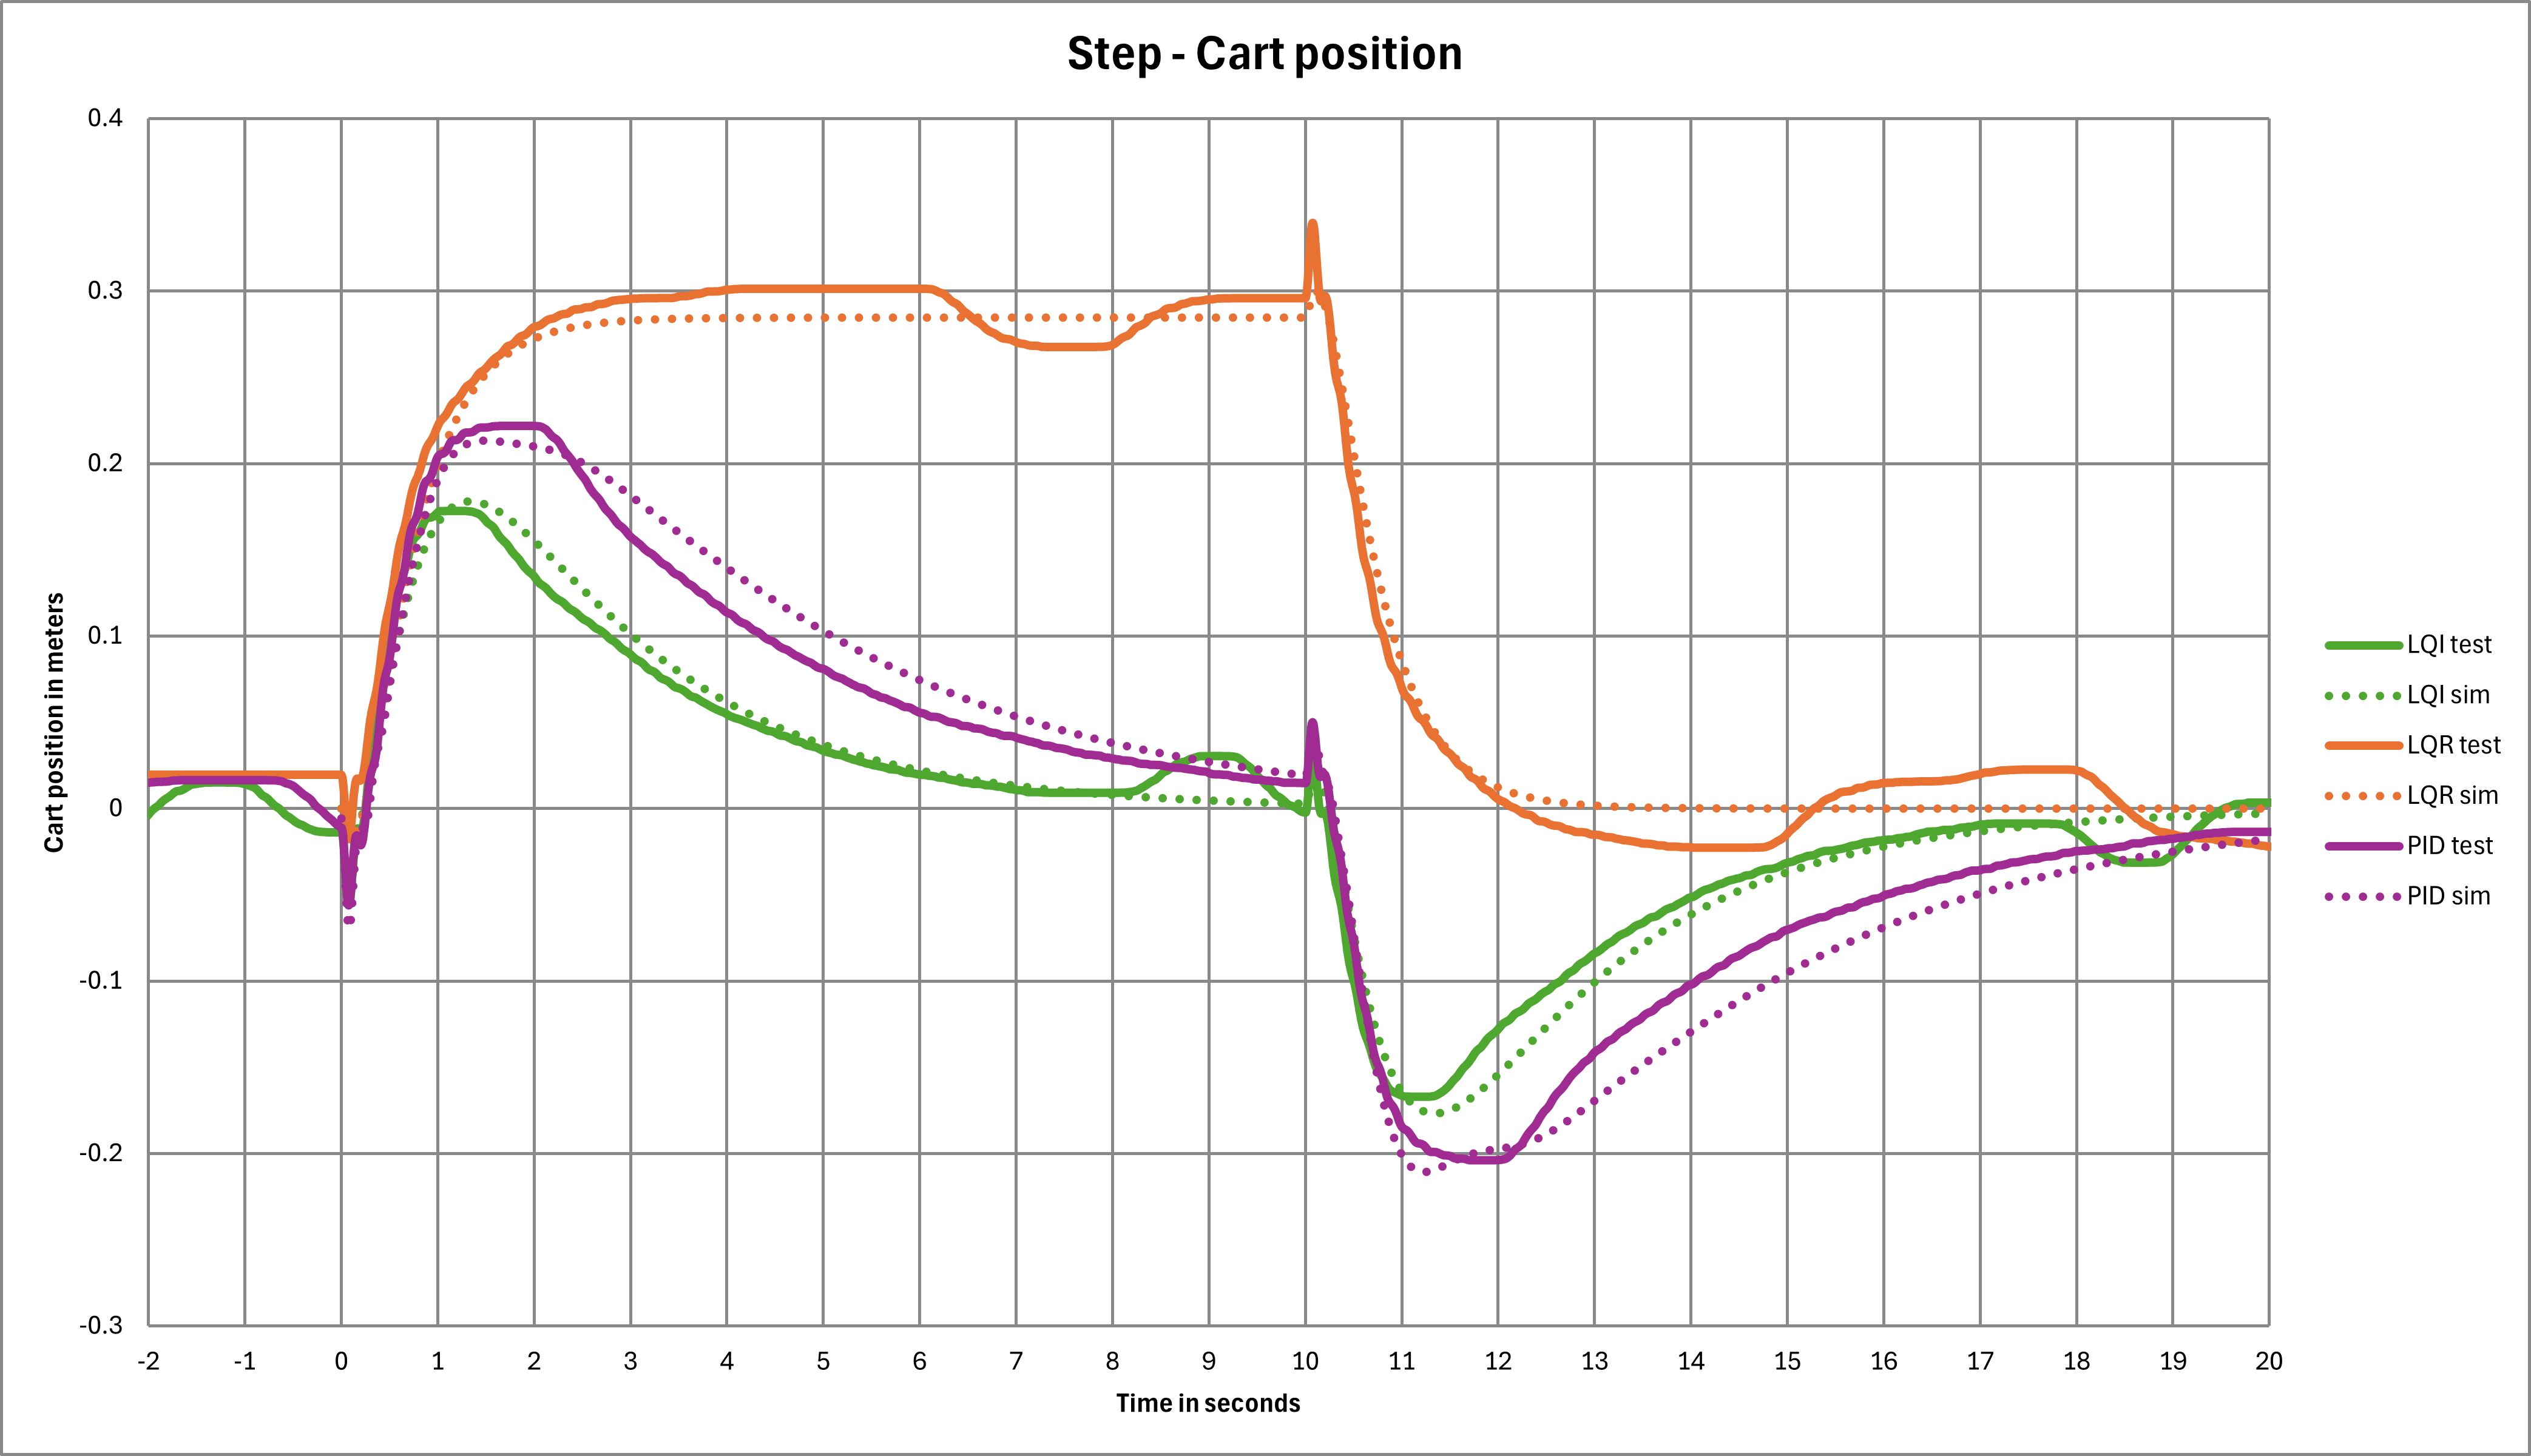
\includegraphics[width=1.0\textwidth]{Figures/Step_cart_pos.png}
	\caption{Cart position during the step response test.}
	\label{fig:Step_cart_pos}   
\end{figure}

\begin{figure}[H]
    \centering
	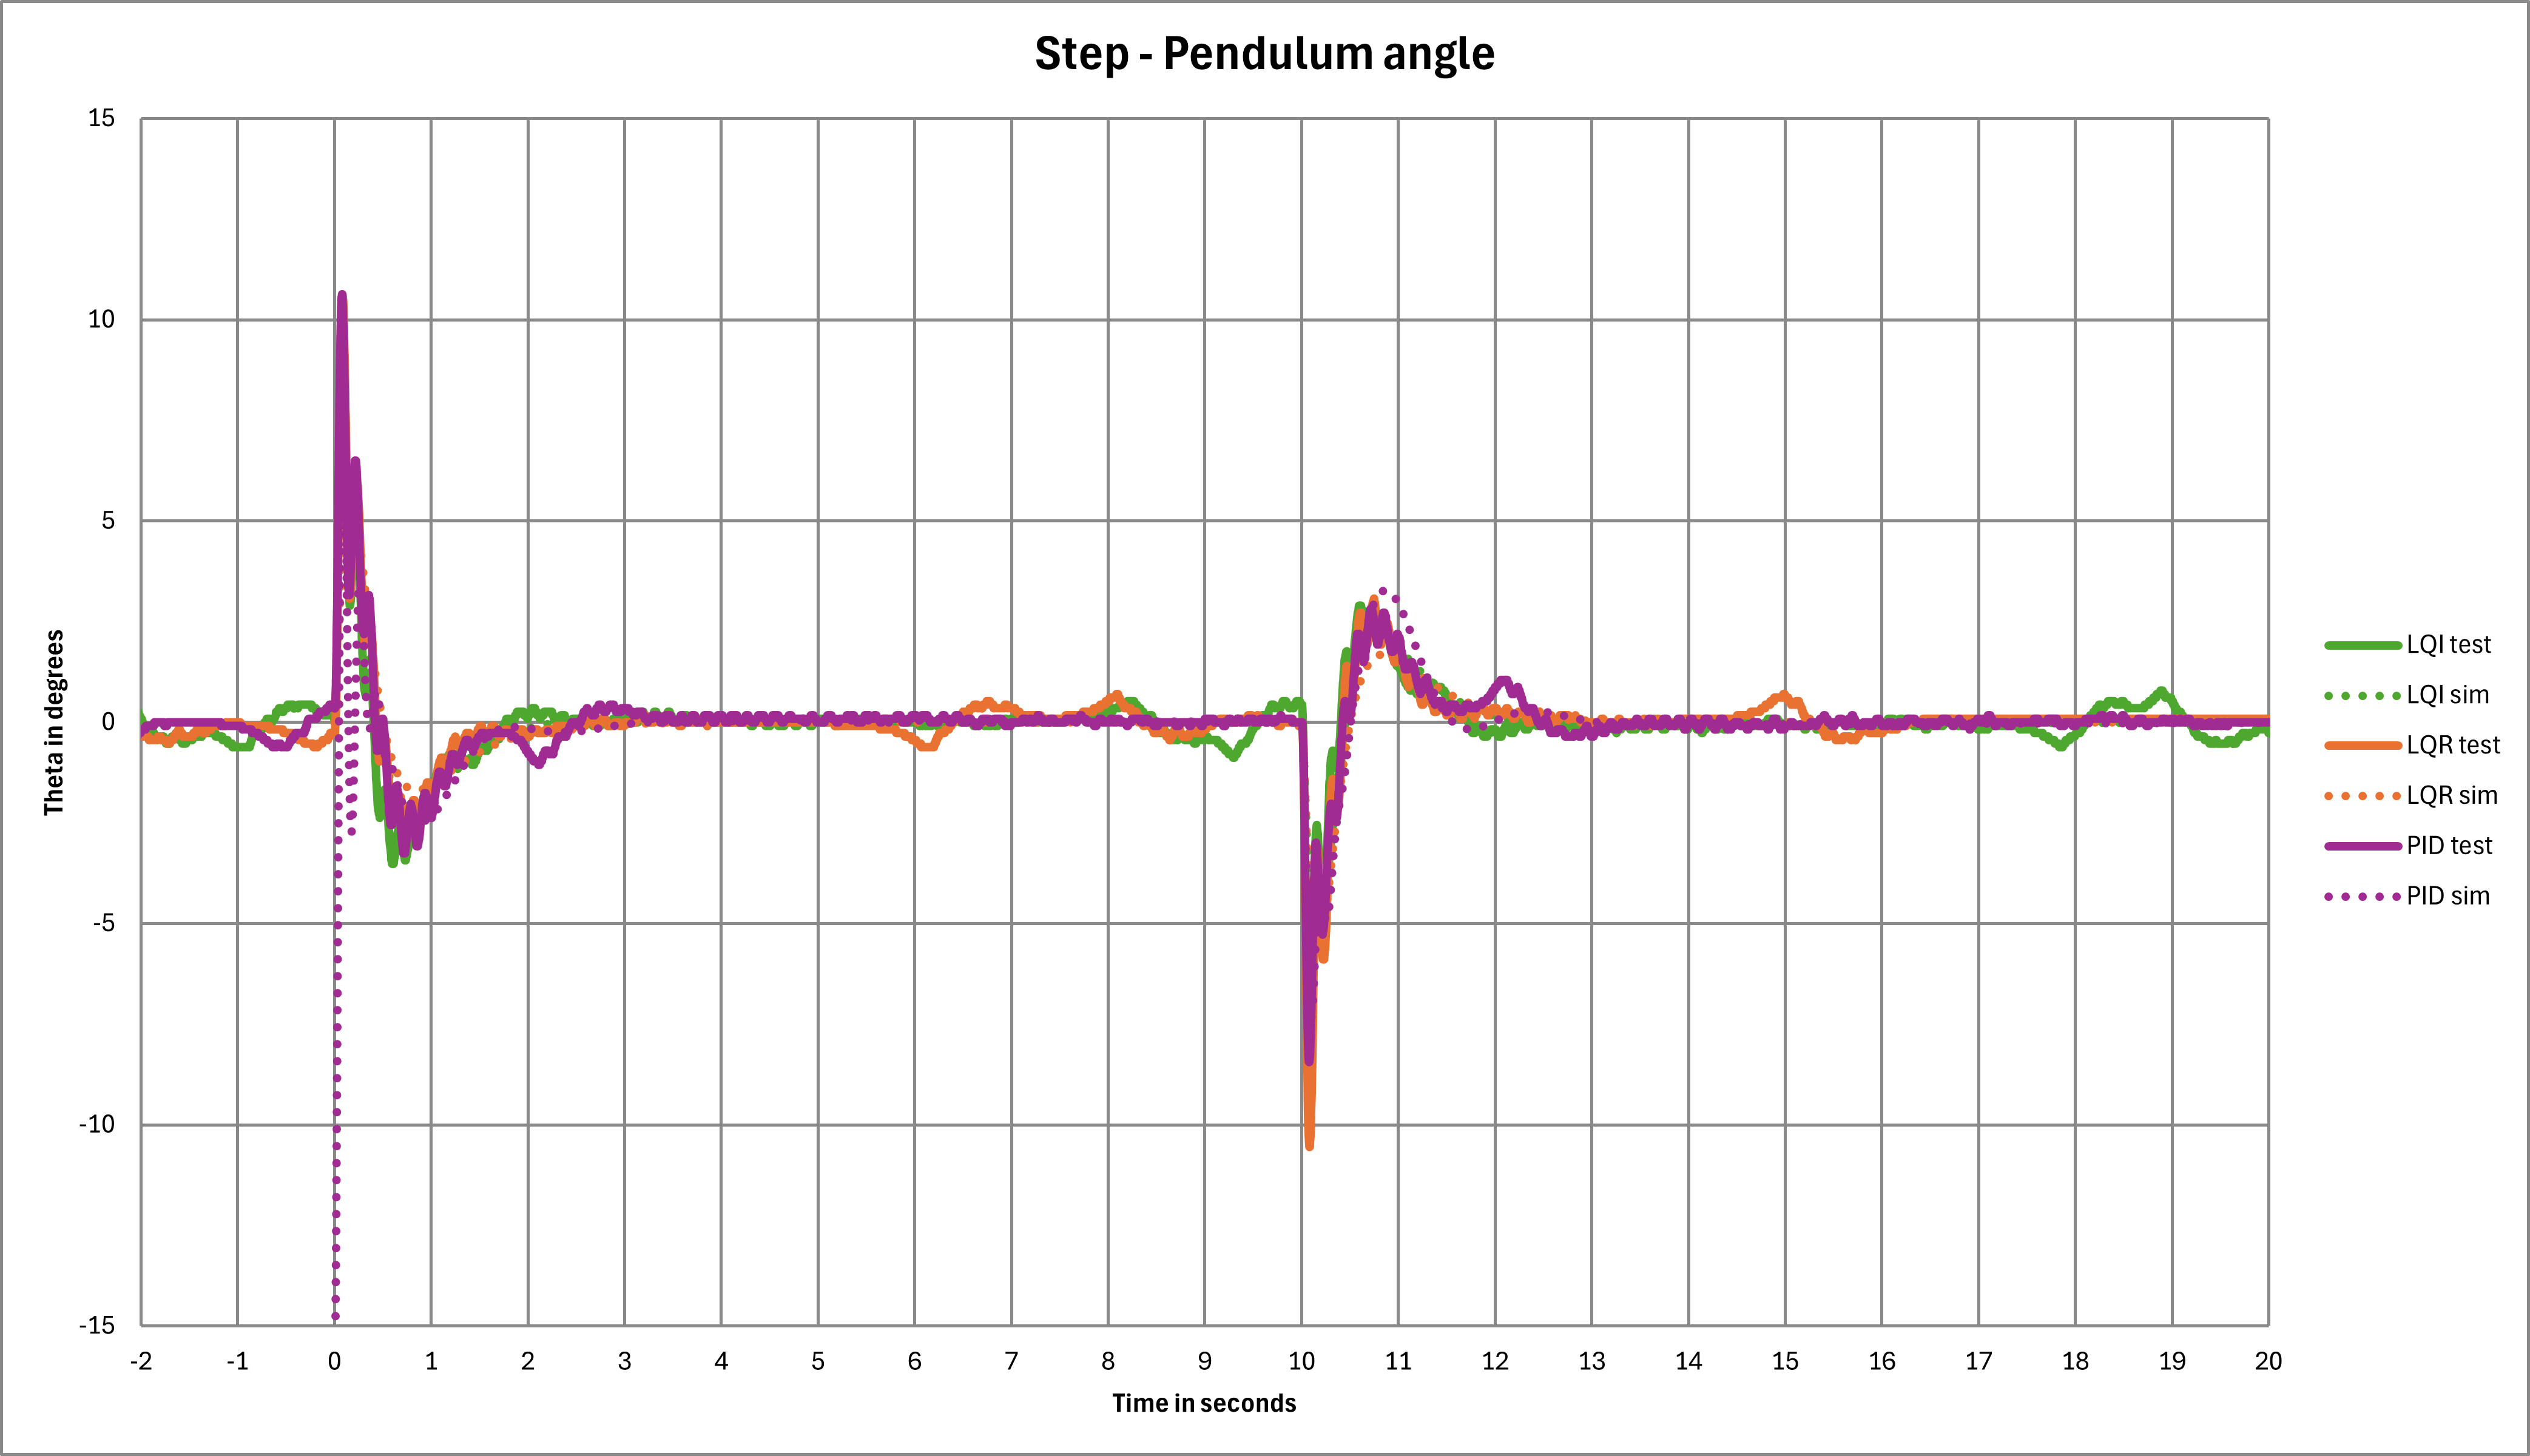
\includegraphics[width=1.0\textwidth]{Figures/Step_pend_angle.png}
	\caption{Pendulum angle during the step response test.}
	\label{fig:Step_pend_angle}   
\end{figure}

\begin{figure}[H]
    \centering
	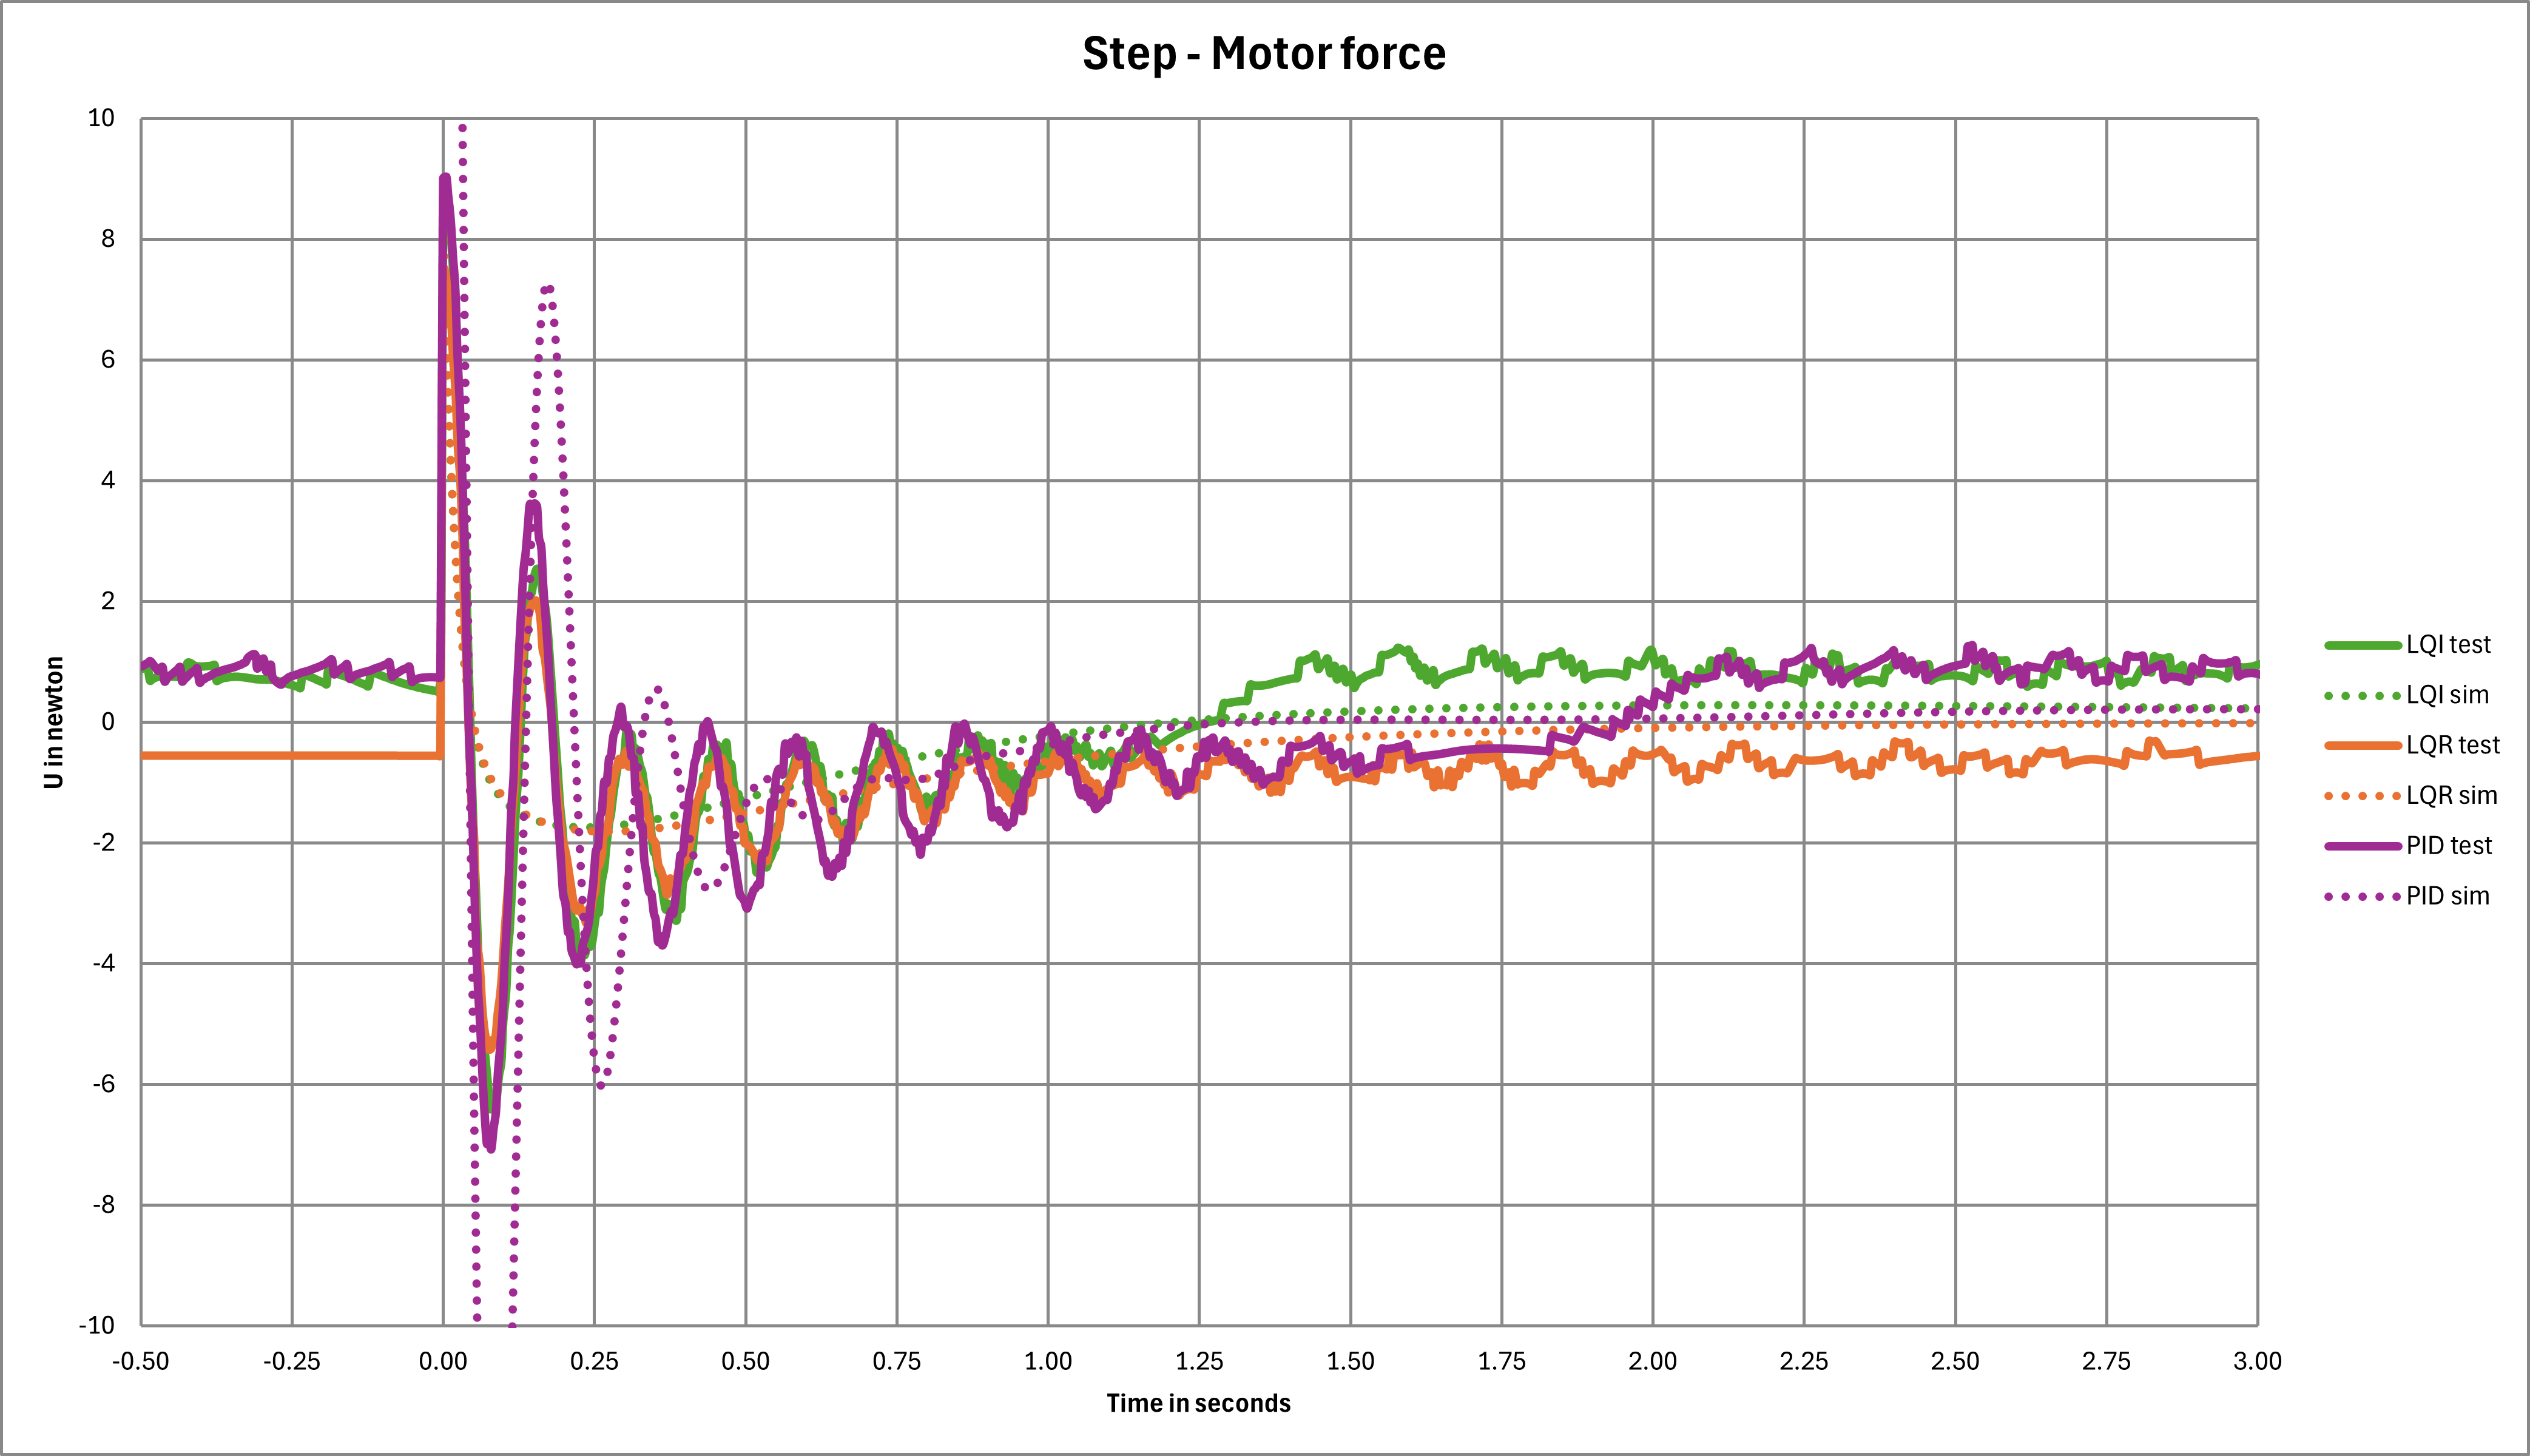
\includegraphics[width=1.0\textwidth]{Figures/Step_motor_u.png}
	\caption{Motor force during the step response test.}
	\label{fig:Step_motor_u}   
\end{figure}


\subsection{Swing up test}

Finally the swing up test, which was done by initiating the swing up, and switching to the controller when possible. This shows how quickly and well the controller can activate, stabilizing an unstable pendulum, and catching it when it reaches the top with a velocity that would allow the given controller to catch it. One thing to note is that the graphs only show the time after the controller kicked in, and not during the swingup itself.

\begin{figure}[H]
    \centering
	
\includegraphics[width=1.0\textwidth]{Figures/Swing_cart_pos.png}
	\caption{Cart position during the swing up test.}
	\label{fig:Swing_cart_pos}   
\end{figure}

\begin{figure}[H]
    \centering
	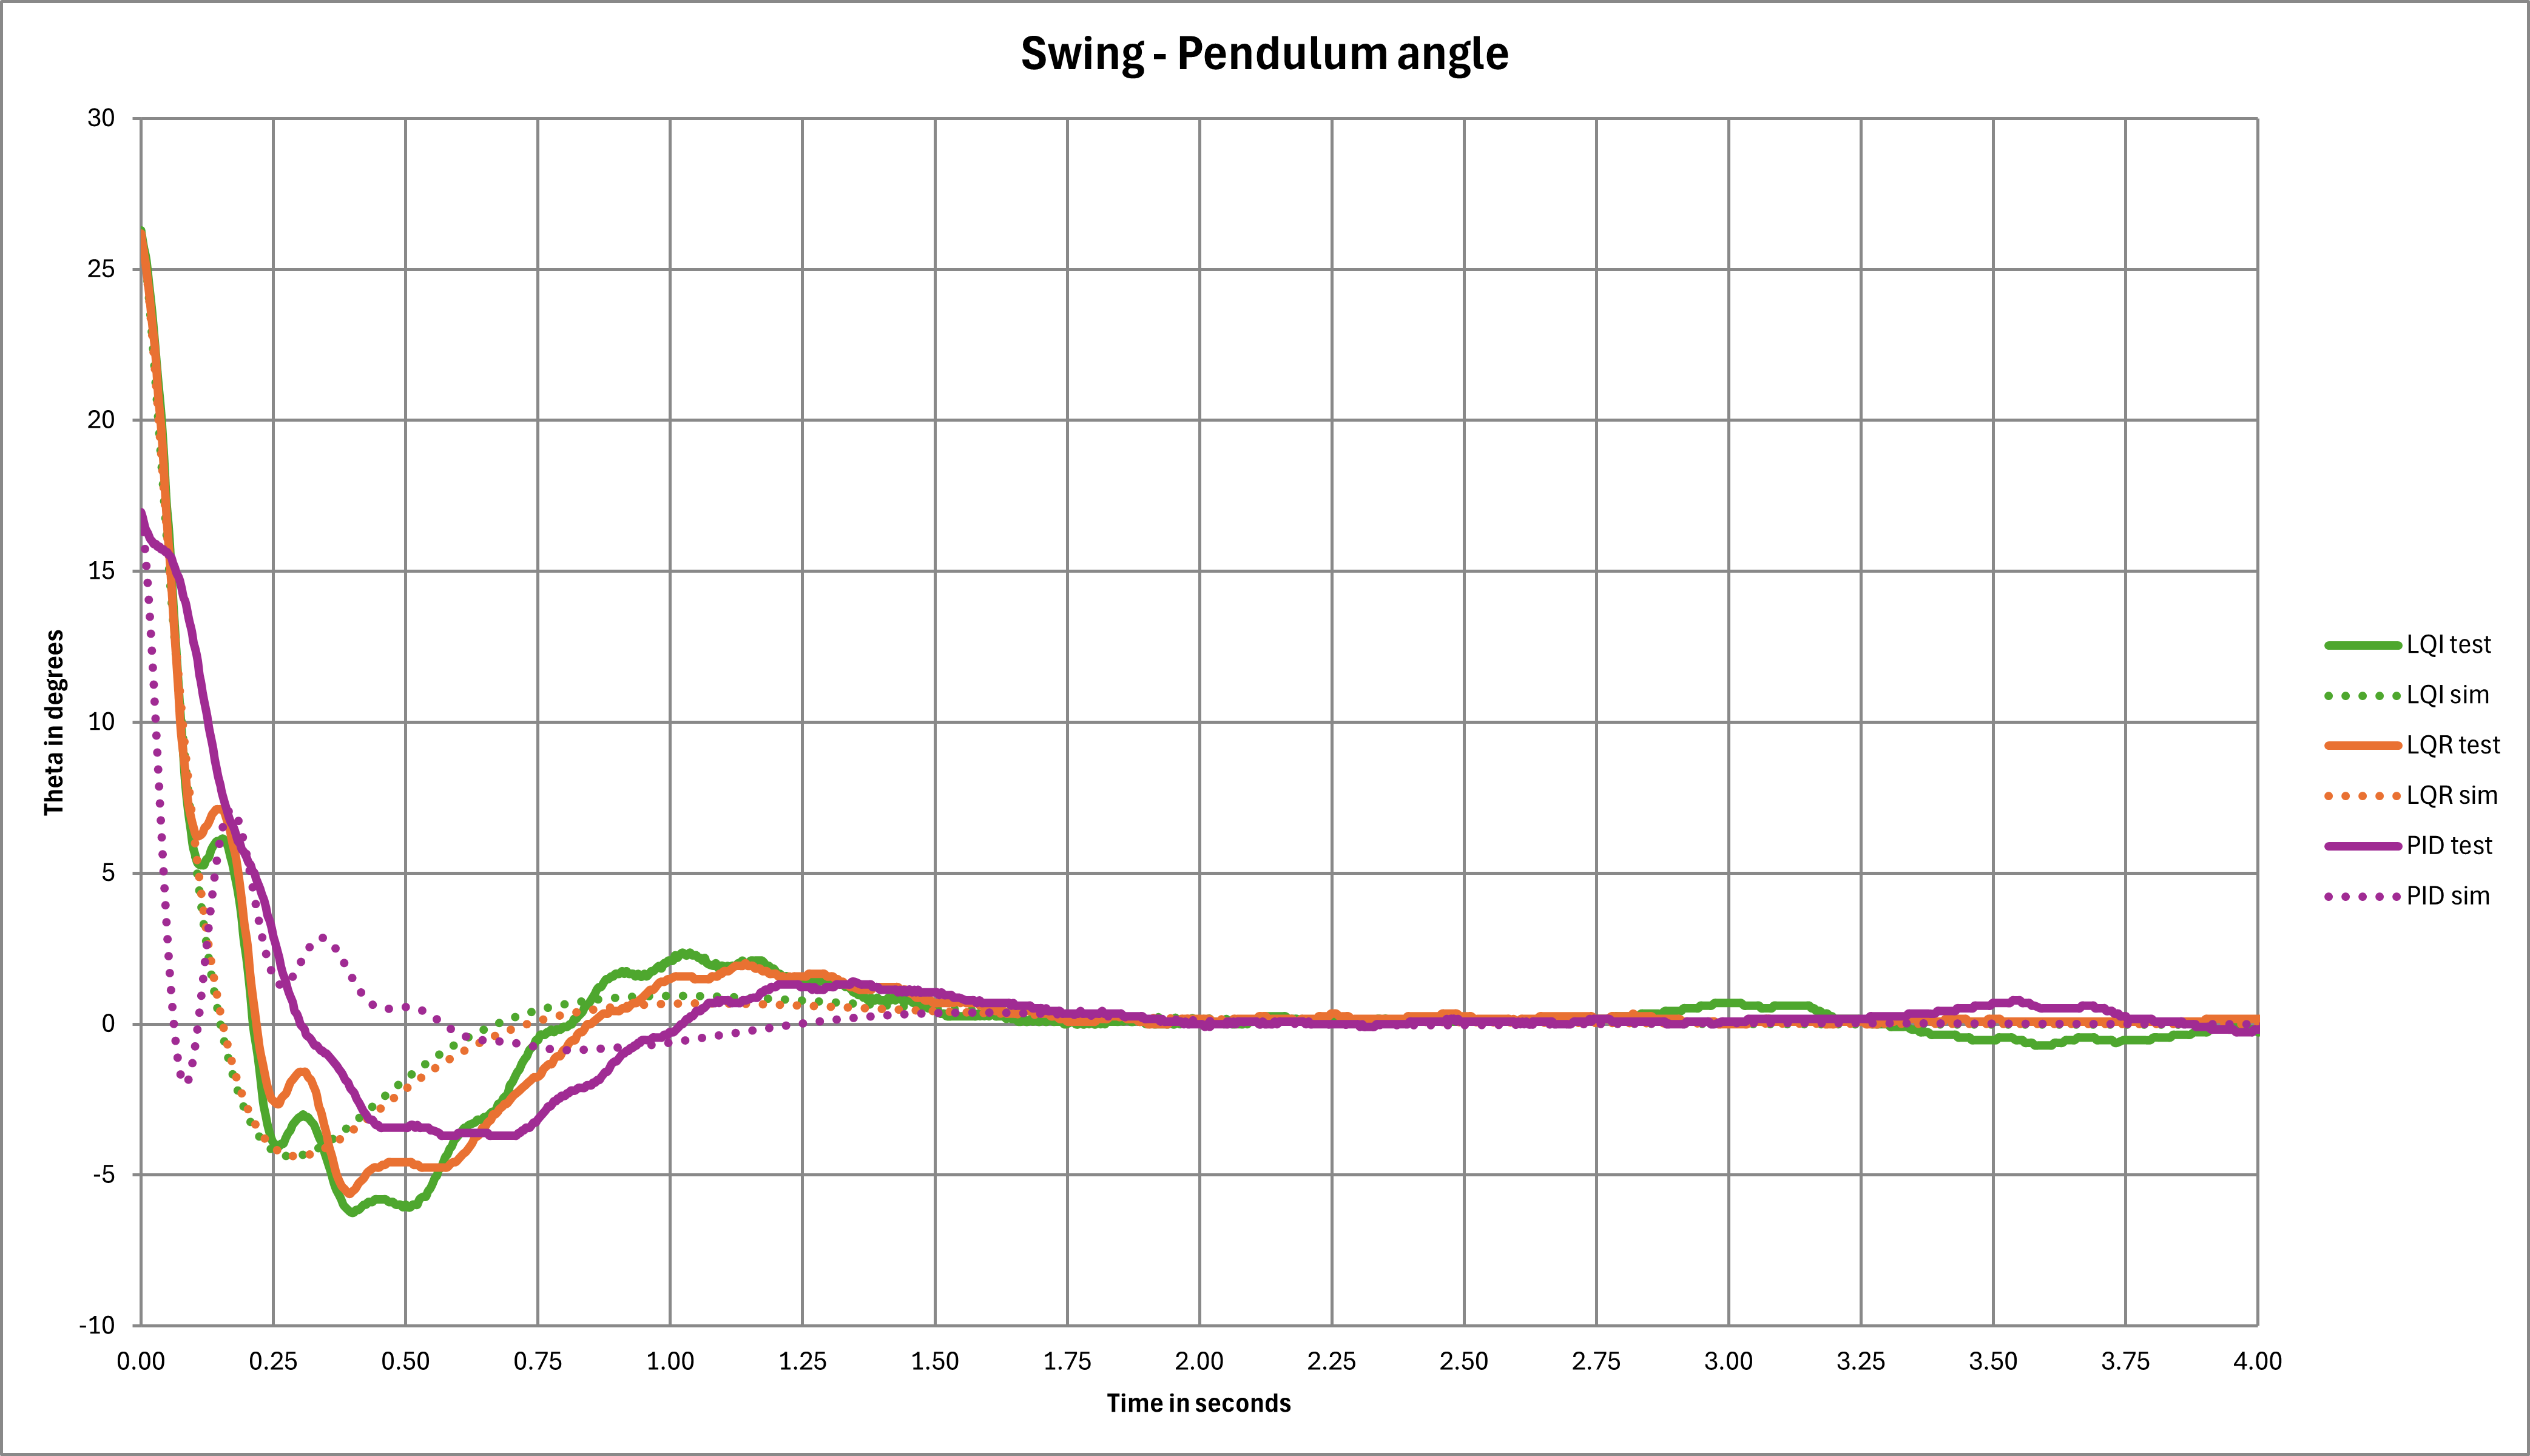
\includegraphics[width=1.0\textwidth]{Figures/Swing_pend_angle.png}
	\caption{Pendulum angle during the swing up test.}
	\label{fig:Swing_pend_angle}   
\end{figure}

\begin{figure}[H]
    \centering
	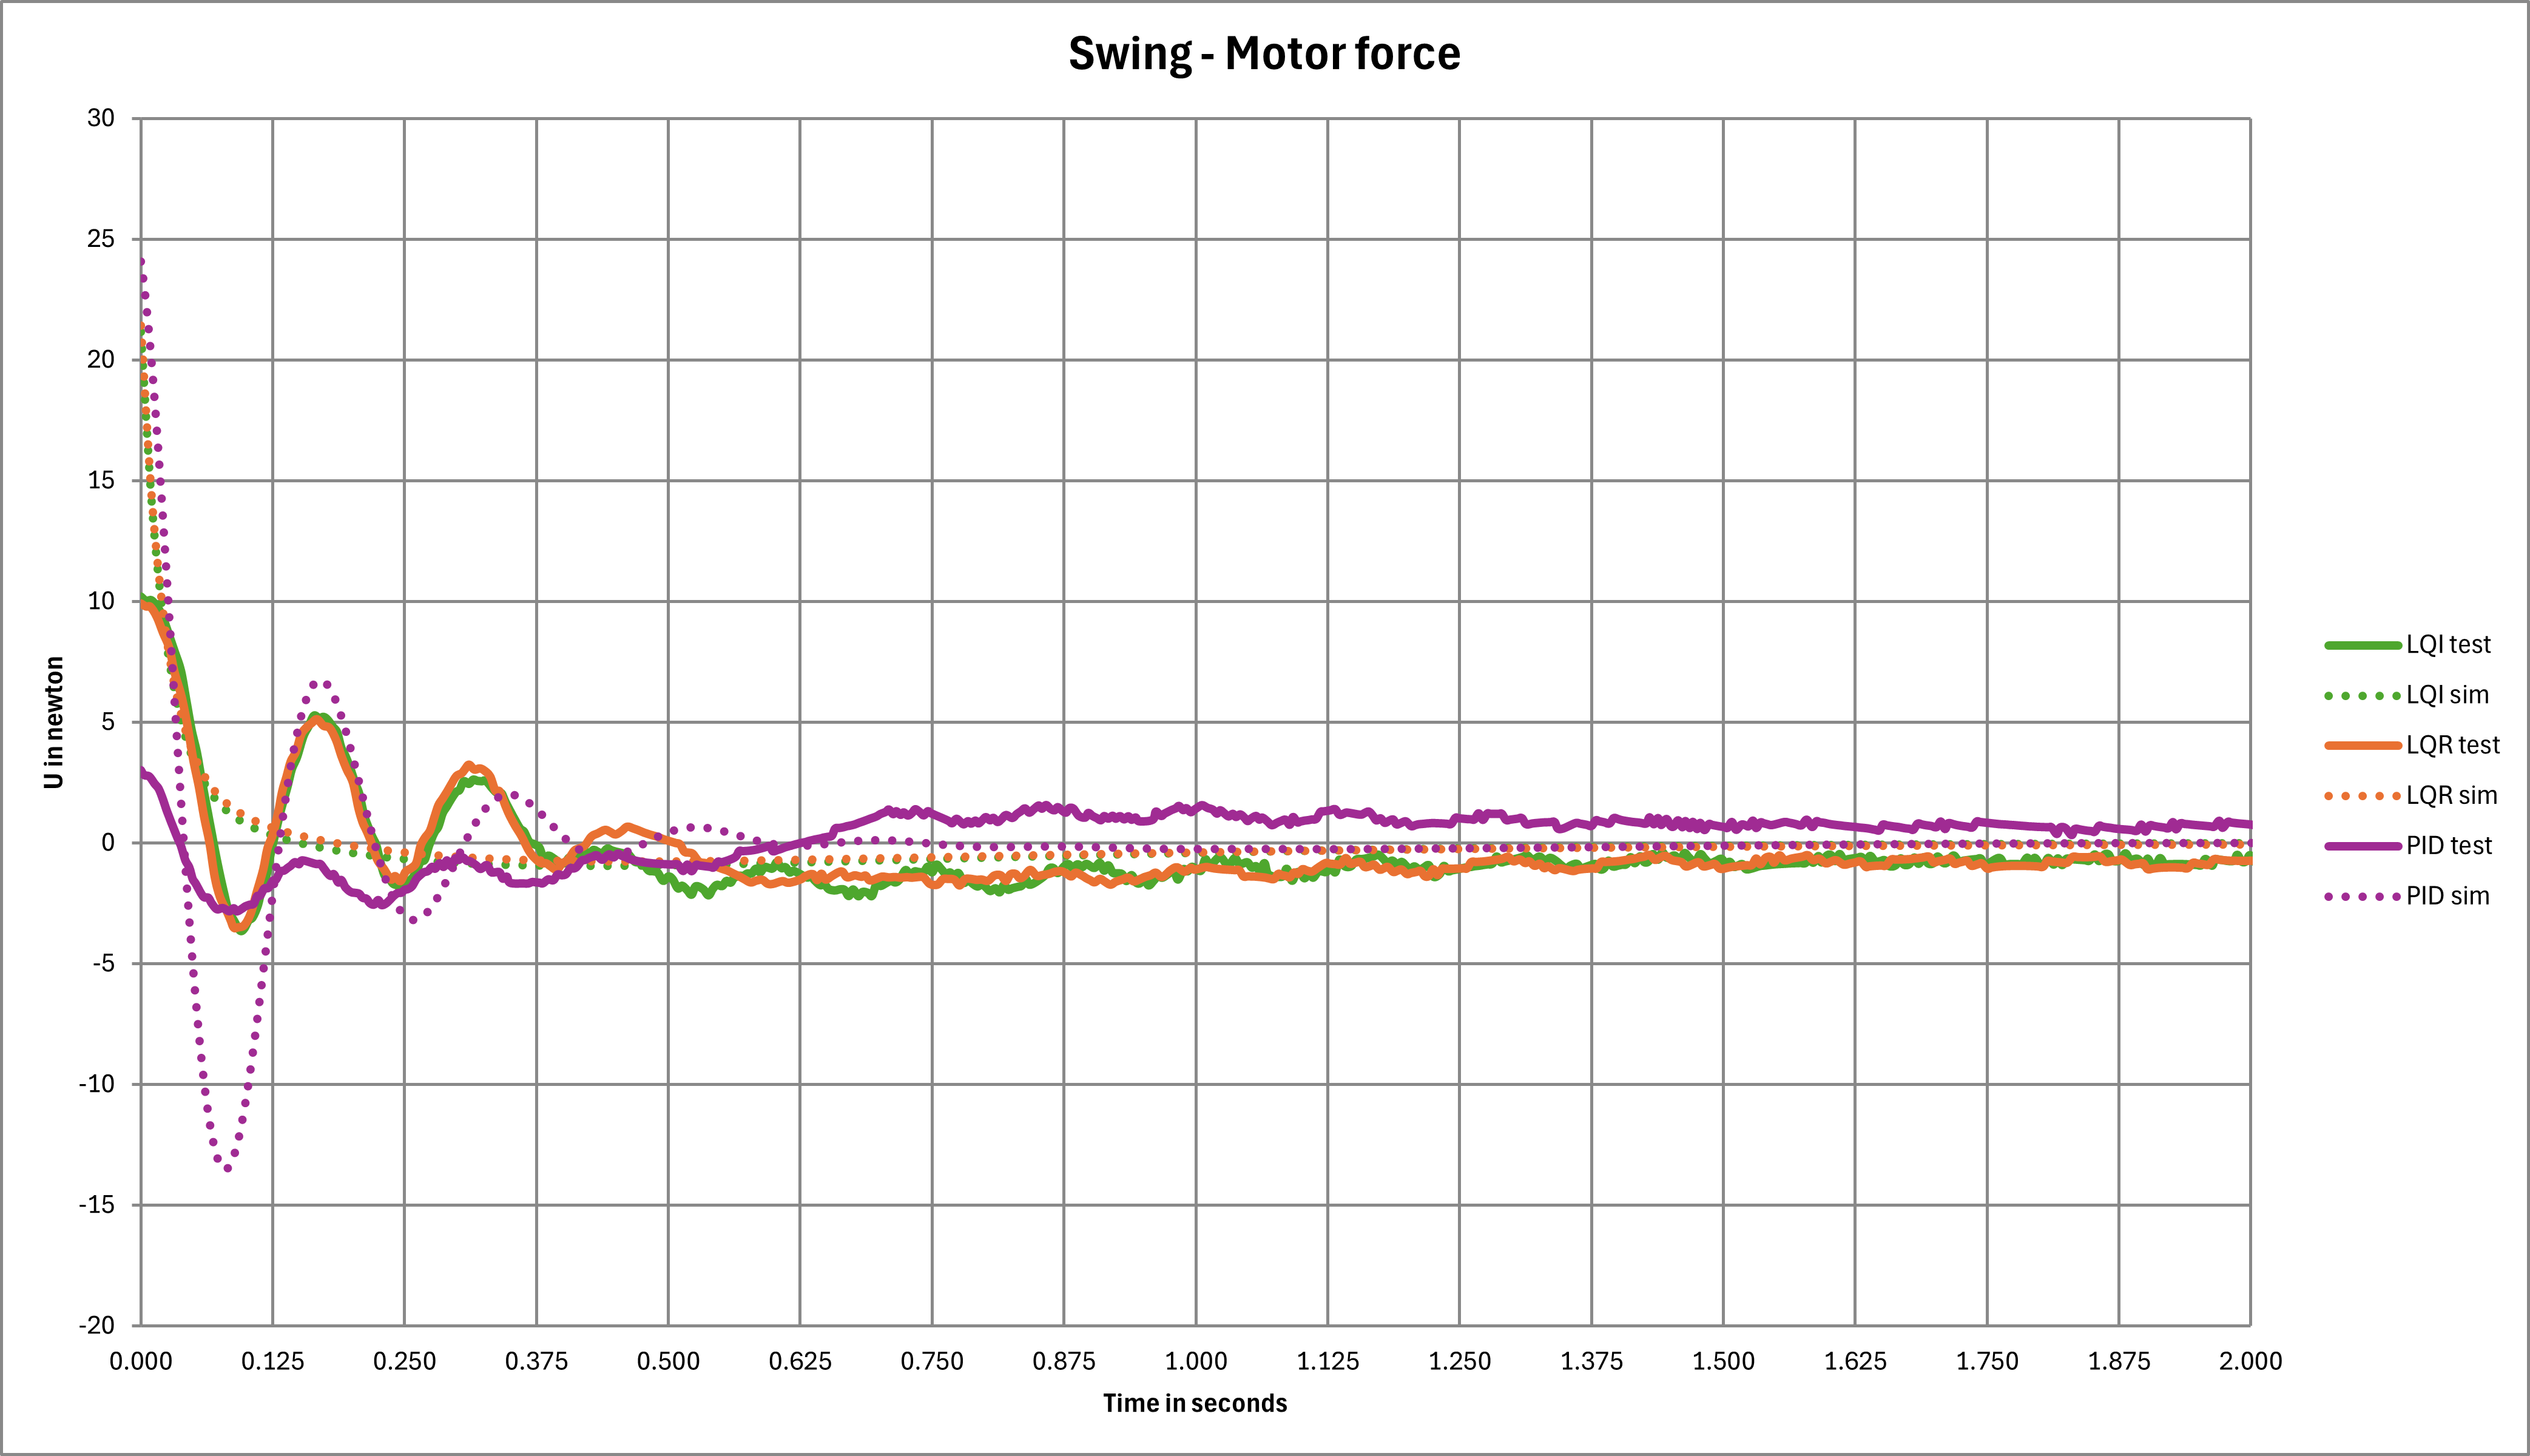
\includegraphics[width=1.0\textwidth]{Figures/Swing_motor_u.png}
	\caption{Motor force during the swing up test.}
	\label{fig:Swing_motor_u}   
\end{figure} 
	\chapter{Discussion}
\label{chap:discussion}

\section{Implementation}

The introduction of a filter on the velocity was found to be necessary during testing. The implementation uses an exponential moving average which can be tuned using a scalar $\alpha$. It is important to note that this is trade-off between noise suppression and phase delay. It was vital in order to limit jittering, while the phase delay did not seem to impact performance to a point of instability even with an $\alpha = 0$.

The implementation of the controllers on the physical system does come with some challenges and limitations. One of the early important factors to consider was the minimum cycle time of the PLC. The default cycle time is set at 10 ms, which quickly showed itself as an issue. With the first attempt at getting a controller to work, a preliminary PID controller was tested at the default cycle time. Unsurprisingly it did not stabilize. After some trial and error, changing parameters, gains and the like, to no avail, it was found that the cycle time was the crucial issue. Lowering it first to 2 ms, got the pendulum somewhat stable. Later the cycle time was pushed to the hardware limit of 1 ms, with a short tolerance for cycle time overshoot. This allows the PLC to continue running its primary loop even if the computation time exceeds the cycle time, with a margin of 10 ms. If the total delay ever got to 10 ms, the loop would stop running. At no point during the testing phase did the PLC shut off due to this computation delay. 

While it was not achievable to get the pendulum stable at a 100 Hz sampling frequency during preliminary testing, it should theoretically be possible. One benefit to using a slower sampling rate is the reduction of noise impact. With a very fast sampling rate, any slight changes and inconsistencies in the data will impact the calculations substantially. A slower rate will act as a natural filter, smoothing some of the noise, but also increasing the delay of information.

\section{Data Collection}
One of the major hardware limitations of the PLC is its storage capacity. This means it is not viable to collect the data directly on the PLC to be moved later. Thus the data must be moved from the PLC to another device continuously, which is why an OPC UA system was implemented. The speed of the OPC UA communication is somewhat limited, and paired with python, slightly fluctuating. This shows itself in the test data as the data points are not collected at a fixed rate. Though the PLC sampled information every millisecond, the collected samples have 3-4 ms between them. In order to counteract this uncertainty, the samples are sent as the last thing during a cycle and a step count from the PLC is sent along with it. This means the state of system should match the step count and should be consistent in each data sample, allowing the data to be synchronized. While this solution is sub-optimal, it was determined to be acceptable for the testing required in this project.
	\chapter{Conclusion}
\label{chap:conclusion}
The purpose of this project was to model, simulate and control an inverted pendulum mounted on a conveyor-driven cart system. The project combined theoretical modelling, controller design, simulation, PLC implementation and experimental validation of the physical setup. Due to the unstable and nonlinear nature of the inverted pendulum system, the project provided both theoretical and practical challenges related to modern control engineering and automation systems.
Mathematical models of the system were developed using both the Newton-Euler and Euler-Lagrange methods. Although the two approaches were derived from different physical principles, both methods resulted in equivalent dynamic models after linearization around the upright equilibrium position. The linearized models were implemented in MATLAB/Python and used for simulation, controller development and performance analysis.
Several controllers were designed and implemented, including LQR, LQI and cascaded PID. In addition, an energy-based swing up controller was implemented to move the pendulum from the downward hanging position into a range where the balancing controllers could stabilize the system. All controllers were successfully implemented on the physical PLC-based setup and were capable of balancing the pendulum under normal operating conditions.
The experimental results showed that the physical system generally behaved similarly to the simulated models, confirming that the developed mathematical models captured the dominant dynamics of the system. However, noticeable differences between simulation and physical behavior were observed during testing. These differences were primarily caused by unmodelled physical effects such as static friction, backlash, sensor noise, filtering delays actuator saturation and small mechanical imperfections in the setup. In particular, static friction in the conveyor system appeared to have a larger impact on the controller behavior than initially expected, especially for the controllers containing integral action.
Among the tested controllers, the LQR controller provided smooth and stable balancing with relatively low oscillation while the LQI controller improved steady-state position regulation through the addition of integral action. The cascaded PID controller was also able to stabilize the pendulum, although it required substantial manual tuning compared to the state-space based controllers. The project furthermore demonstrated several practical implementation challenges related to real-time control systems including PLC cycle time limitations, encoder quantization, OPC UA communication delays and noisy velocity estimation.
Overall, the project succesfully demonstrated both the theoretical and practical aspects of modelling and controlling an unstable dynamic system. The developed controllers achieved stable balancing of the inverted pendulum and the project provided valuable insight into dynamic modelling, simulation, controller implementation and real-world automation system integration.
	\cleardoublepage
\addcontentsline{toc}{chapter}{References}
\renewcommand{\bibname}{References}
\begin{thebibliography}{99}
	
	\bibitem{Servomotor}
	Schneider Electric,
	AC Servomotor BSH0552T01A2A,
	Last accessed 28.05.2026. \\
	Available at: \url{https://www.se.com/dk/da/product/BSH0552T01A2A/ac-servomotor-bsh-0-9-n-m-6000-rpm-uden-bremse-ip50/}
	
	\bibitem{Servo Drive}
	Schneider Electric,
	Lexium 32C Servo Drive,
	Last accessed 28.05.2026. \\
	Available at: \url{https://www.se.com/in/en/download/document/0198441113761-EN/}
	
	\bibitem{PLC}
	B\&R Industrial Automation, 
	Programmable Logic Controller X20CP1382, 
	Last accessed 28.05.2026. \\
	Available at: \url{https://bippa.ru/upload/iblock/522/ge8hmgplesp451nxbu1bmv42slwqn1yq/X20CP1382-en.pdf}
	
	\bibitem{System parameters}
	Cheng Fang,
	Lecture Notes: \emph{System parameters},
	Maj 2026,
	Available on ItsLearning
	
	\bibitem{Newton euler}
	Christoffer Sloth,
	Lecture Notes: \emph{Lektion 3. Bevægelse og kræfter},
	Februar 2026,
	Available on ItsLearning
	
	\bibitem{Euler-lagrange}
	Christoffer Sloth,
	Lecture Notes: \emph{Lektion 11: Euler-Lagragne modellering},
	Februar 2026,
	Available on ItsLearning
	
\end{thebibliography}

	
	\appendix
	\newpage
\begingroup
\renewcommand{\clearpage}{}

\chapter{Distribution of Tasks}
\label{chap:taskdistribution}

\begin{table}[h!]
	\centering
	\caption{Distribution of Tasks}
	\label{tab:dot}
	\begin{tabular}{lccccc}
		\toprule
		\textbf{Task} & \textbf{Noah} & \textbf{Rasmus} & \textbf{Emma} & \textbf{Jannick} & \textbf{Eymundur} \\
		\midrule
		\multicolumn{6}{c}{Development} \\
		\midrule
		\textbf{System Modeling} & & & x & x & x \\
		\textbf{Control Theory} & & & & x & x \\
		\textbf{PLC Implementation} & & x & & & \\
		\textbf{Data Collection} & x & & & & x \\
		\midrule
		\multicolumn{6}{c}{Report} \\
		\midrule
		\textbf{Abstract} & x & x & x & & \\
		\textbf{Introduction} & & & x & & \\
		\textbf{System Modeling} & & & x & & \\
		\textbf{Control Theory} & & & & x & \\
		\textbf{PLC Implementation} & & x & & & \\
		\textbf{Data Collection} & x & & & & x \\
		\textbf{Results} & x & x & & &\\
		\textbf{Discussion} & & x & & x & x \\
		\textbf{Conclusion} & & & x & & \\
		\bottomrule
	\end{tabular}
\end{table}

\chapter{Code}
\label{chap:code}

The code is available in the attached ZIP file as well as on github at: \\

\chapter{Video Showcase}
\label{chap:videoshowcase}

A video of the system running is available at: \\

\endgroup

	
\end{document}
